\section{Datenhaltung}
Die App muss sich um die Verwaltung von Accountdaten, Einstellungen, Videos, Metadaten und symmetrischen Schlüsseln kümmern. 

\subsection{Nutzerdaten}
Für Accountdaten und  Einstllungen bieten sich die von Android bereitgestellten SharedPreferences an, die als Key-Value-Pairs aufgebaut werden. Das Schema ist in Schaubild \ref{fig:sharedpreferences_overview} veranschaulicht. Der Key entspricht den Daten die abgefragt werden sollen, also Einstellungen oder Account. Die gelesenen Werte bestehen jeweils aus einem String im JSON Format. Dadurch erreicht man eine Bündelung aller zusammengehörender Werte unter einem Key, unterstützt die Änderbarkeit und Ergänzbarkeit bestehender Daten und vereinfacht die Instanziierung von Account- und Einstellungen-Objekten durch einen Konstruktor, der einen JSON String entgegennimmt.\newline\par

\begin{figure}[ht]
	\centering
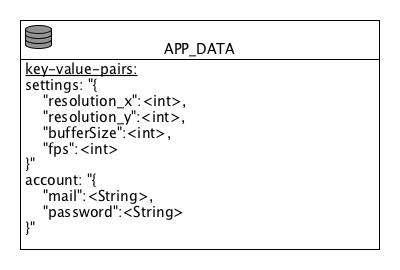
\includegraphics[width=0.5\textwidth]{./resources/Diagramme/App/SharedPreferences_overview.jpg}
\caption{Key-Value-Pairs der SharedPreferences}
	\label{fig:sharedpreferences_overview}
\end{figure}

\subsection{Dateien}
Für die Speicherung von Videos, Metadaten und symmetrischen Schlüsseln erweisen sich die SharedPreferences jedoch als ungeeignet. Hier gibt es zwei Lösungen: Entweder man speichert sie im internen oder im externen Speicher. Wir werden die erste Variante wählen, werden uns aber die Möglichkeit zum Exportieren der Daten in den externen Speicher frei halten. Der naive Ansatz merkt sich in den oben beschriebenen SharedPreferences die Namen aller gespeicherten Dateien und referenziert sie dadurch. Dabei ergibt sich aber folgendes Problem: Nachdem der Nutzer alle appinternen Daten gelöscht hat, hat man keine Chance mehr an extern gespeicherte Daten zu kommen. \newline\par
Wir verwenden einen generischeren Ansatz, der gänzlich auf die verwendung der SharedPreferences verzichtet: Es existieren drei Ordner: Ein Video-, ein Metadata- und ein Keyordner. Jedes Video erhält einen eindeutigen Namen, bestehend aus der exakten Aufnahmezeit. Jede mit diesem Video verwandte Datei, also dessen Metadaten und Schlüssel, besitzen den gleichen Dateinamen.\newline\par

Bezüglich der Metadaten muss auch beachtet werden, dass sie über die App ausgelesen werden können müssen, sie jedoch beim Speichervorgang des Videos direkt verschlüsselt werden um sie beim Hochladen des Videos verschlüsselt übertragen zu können. Aus diesem Grund werden die Metadaten in zwei Inhaltlich identische Dateien abgelegt. Eine der beiden wird veschlüsselt, die Andere nicht. An den Dateinamen der unverschlüsselten Datei wird zur identifikation schließlich ``\_readable'' angehängt\newline\par

Zusätzlich zu den erwähnten Ordnern existiert ein weiterer Ordner, der verwendet wird, um temporäre Videodateien abzulegen. Unter einer temporäre Videodatei ist hier ein unverschlüsseltes Video zu verstehen, welche nur zwischengespeichert wird. Android bietet hierzu die Möglichkeit, die temporäre Datei im appinternen Cache-Ordner abzulegen. Dies bietet außerdem den Vorteil, dass nur die App selbst Zugriff darauf hat.

